% !TeX root = ..\G16.tex
\section{Implementering}

\subsection{Board}\label{sec:boardImplement}
Modellen for brættet implementeres i \mintinline{java}|Board.java| klassen. \cref{tbl:boardfields} indeholder klassens felter.
\begin{table}[H]
    \centering
    \caption{Felter i \mintinline{java}|Board.java|}\label{tbl:boardfields}
    \begin{tabular}{ll}
        \toprule
        Felt                                                              & Formål                                           \\
        \midrule
        \mintinline{java}|int[][]board|                                   & Datastruktur der repræsenterer brættet.          \\
        \mintinline{java}|int turnCount|                                  & Turnummeret i spillet                            \\
        \mintinline{java}|int boardsize|                                  & Størrelsen \(n\) for et \(n\times n\) bræt.      \\
        \mintinline{java}|int forfeitCounter|                             & Antal gange en spillerne har meldt pas           \\
        \mintinline{java}|ArrayList<int[]> flipped|                       & Log over de sidste vendte brikker                \\
        \mintinline{java}|HashMap<Integer, String> players|               & Spillernes interne ID og navne                   \\
        \mintinline{java}|HashMap<String, HashMap<Integer,|               & Datastruktur for mulige træk for en given farve, \\
        \quad \mintinline{java}|HashMap<Integer, Integer[]>>> validMoves| & en given tur.                                    \\
        \bottomrule
    \end{tabular}
\end{table}
Brættet repræsenteres af en heltalsmatrix med værdierne \(0\) for tomt felt, \(1\) for hvid placering og \(2\) for sort placering. Ved at gemme turnumre og antal gange spillere har meldt pas kan board klassen afgøre hvis tur det er og om spillet er slut.
Loggen over vendte brikker endte med ikke at blive brugt, men formålet var at kontrollerklassen skulle vise hints om hvilke brikker der ville blive vendt ved et givent træk. Det blev stemt ned da det gør spillet for nemt.\newline
\cref{tbl:boardmethods} indeholder klassens metoder.
\begin{table}[H]
    \centering
    \caption{Metoder i \mintinline{java}|Board.java|}\label{tbl:boardmethods}
    \begin{tabular}{ll}
        \toprule
        Metode                                                        & Formål                                                                \\
        \midrule
        \mintinline{java}|Board()|                                    & Konstruktør for brættet. Kalder \mintinline{java}|setPlayers()|.      \\
        \mintinline{java}|getBoard()|                                 & Getter for board feltet.                                              \\
        \mintinline{java}|setPiece(int row, int column, int colour)|  & Sætter manuelt brik, uanset lovlighed.                                \\
                                                                      & Bruges til unit tests.                                                \\
        \mintinline{java}|getTurn()|                                  & Getter for turnCount.                                                 \\
        \mintinline{java}|turnClock()|                                & Inrementere turnCount.                                                \\
        \mintinline{java}|getPlayers()|                               & Getter for spiller hashmap.                                           \\
        \mintinline{java}|getValidMoves()|                            & Getter for validMoves hashmap.                                        \\
        \mintinline{java}|setPlayers()|                               & Tildeler tilfældigt spillere en farve.                                \\
        \mintinline{java}|setPlayers(int id1, String player1,|        & Tildeler spillere specifikke farver.                                  \\
        \quad \mintinline{java}|int id2, String player2)|             &                                                                       \\
        \mintinline{java}|setPlayerName()|                            & Setter for specifikt spillernavn.                                     \\
        \mintinline{java}|resetBoard()|                               & Nulstiller brættet, turnummer og pastæller.                           \\
        \mintinline{java}|turnState(int colour)|                      & Kalder \mintinline{java}|moveAnalyser(colour)|,                       \\
                                                                      & og udregner om der er ledige træk.                                    \\
        \mintinline{java}|gameOver()|                                 & Afgør om spillet er slut hvis brættet er fyldt,                       \\
                                                                      & eller der er meldt pas to gange i træk.                               \\
        \mintinline{java}|initPlace(int row, int column, int colour)| & Indeholder logik for at udfylde startfelterne.                        \\
        \mintinline{java}|place(int row, int column, int colour)|     & Placere en brik hvis placeringen er tom og                            \\
                                                                      & indeholdt i validMoves. Kalder \mintinline{java}|flip(move, colour)|. \\
        \mintinline{java}|flip(String move, int colour)|              & Vender brikker ved et lovligt træk.                                   \\
        \mintinline{java}|filled()|                                   & Afgører om brættet er fyldt.                                          \\
        \mintinline{java}|checkWinner()|                              & Tæller brikker og afgører vinderen.                                   \\
        \mintinline{java}|moveAnalyser(int colour)|                   & Finder lovlige træk (se \cref{sec:moveAnalyser}).                     \\
        \mintinline{java}|findOwn(int[][] checkboard, int i,|         & Findere mulig indkapsling af modstanderen.                            \\
        \quad \mintinline{java}|int j, int direction, int colour)|    &                                                                       \\
        \mintinline{java}|saveFlips(int[] ownPiece, int i,|           & Gemmer indkapslede brikker.                                           \\
        \quad \mintinline{java}|int j, int direction)|                &                                                                       \\
        \bottomrule
    \end{tabular}
\end{table}
De fleste metoder er simple if/else eller for-løkker, og de er vel dokumenterede i kildekoden.\newline
Den vigtigste funktion i \mintinline{java}|Board.java| er \mintinline{java}|moveAnalyser(int colour)| metoden som skal finde og afgører alle træks lovlighed for et givent bræt setup og en given brikfarve. Metoden gennemgås i \cref{sec:moveAnalyser}.
\subsubsection{AdvancedReversi board klasse}
Der er enkelte ændringer i den avancerede udgave af spillet. \mintinline{java}|setPlayers()| metoden ændres til ikke at foretage tilfældige valg, da brugeren selv skal skrive navne ind i systemet. Pastælleren, \mintinline{java}|gameOver()| og \mintinline{java}|filled()| fjernes helt, for at overlade denne logik til controller klassen da dette bliver en mere integreret del af brugerinteraktionen. Til gengæld introduceres to metoder: \mintinline{java}|checkBlackScore()| og \mintinline{java}|checkWhiteScore()| som bruges til at live-opdatere optaget terræn for de to spillere.
\subsubsection{\texorpdfstring{\mintinline{java}|moveAnalyser()| metoden og \mintinline{java}|validMoves| feltet}{moveAnalyser() metoden og validMoves feltet}}\label{sec:moveAnalyser}
Flere gange i løbet af spillets afvikling er det praktisk at vide om hvilke træk der er lovlige for en given farve. Betragt \cref{fig:directions}. Her ses at en vilkårlig brik har 8 nabofelter. Særtilfælde er i kanten af brættet. For at undgå særtilfælde blev første implementationsvalg her at udfører alle tests i et bræt med \emph{padding.} Derfor starter validMoves ud med at lave en kopi af brættet med en kant af nuller.
\begin{figure}[H]
    \caption{En briks naboer}\label{fig:directions}
    \begin{align*}
        \begin{array}{ccccc}
            2 &            & 2          &             & 2 \\
              & \nwarrow   & \uparrow   & \nearrow    &   \\
            2 & \leftarrow & 1          & \rightarrow & 2 \\
              & \swarrow   & \downarrow & \searrow    &   \\
            2 &            & 2          &             & 2
        \end{array}
    \end{align*}
\end{figure}

Herefter itererer metoden over alle felter i brættet. Mødes et tomt felt testes alle 8 retninger for en modstander. Hver retning har sin egen heltalskode. Hvis der er en modstander itererer metoden i den retning og leder efter en brik af egen farve for at fastslå en indkapslingsmulighed, med metoden \mintinline{java}|findOwn()|. Hvis metoden støder på kanten af brættet eller en tom placering indstilles søgningen. Dennes algoritme beskrives mere grafisk i \cref{fig:findOwn}.
\begin{figure}[H]
    \centering
    \caption{\mintinline{java}|findOwn()| leder efter en indkapsling i nordvestlig retning (heltalskode 1).}\label{fig:findOwn}
    \begin{subfigure}[t]{.3\textwidth}
        \caption{Første skridt}
        \begin{align*}
            \begin{array}{cccc}
                \color{blue}1 & 0 & 0               & 0             \\
                0             & 2 & 0               & 0             \\
                0             & 0 & \color{DTUred}2 & 0             \\
                0             & 0 & 0               & \color{blue}1
            \end{array}
        \end{align*}
    \end{subfigure}
    \quad
    \begin{subfigure}[t]{.3\textwidth}
        \caption{Andet skridt}
        \begin{align*}
            \begin{array}{cccc}
                \color{blue}1 & 0               & 0               & 0             \\
                0             & \color{DTUred}2 & 0               & 0             \\
                0             & 0               & \color{DTUred}2 & 0             \\
                0             & 0               & 0               & \color{blue}1
            \end{array}
        \end{align*}
    \end{subfigure}
\end{figure}
Den fundne nabobriks koordinater gemmes og returneres til validMoves. Hvis validMoves modtager sådan et koordinat iværksættes saveFlips som gemmer de indkapslede brikker i et hashmap efter samme skridt som i \cref{fig:findOwn}. Her vil de røde brikkerks koordinater blive gemt.\newline
Når validMoves har et hashmap med hashmaps af koordinater fra alle retninger gemmes disse i validMoves hashmappet med trækkets koordinat som nøgle. \cref{tbl:hashmaps} viser strukturen af validMoves.
\begin{table}[H]
    \centering
    \caption{Datastrukturen \mintinline{java}|validMoves| efter afsøgningen i \cref{fig:findOwn}}\label{tbl:hashmaps}
    \begin{tabular}{ccc}
        \toprule
        Træk                               & Retning                             & Vendbare brikker                                 \\
        \midrule
        \mintinline{java}|HashMap<String,| & \mintinline{java}|HashMap<Integer,| & \mintinline{java}|HashMap<Integer, Integer[]>>>| \\
        \multirow{2}{*}{"3,3"}             & \multirow{2}{*}{1}                  & 0, \{2,2\}                                       \\
                                           &                                     & 1, \{1,1\}                                       \\
        \bottomrule
    \end{tabular}
\end{table}
Årsagen til at retning indgår som nøgle i validMoves er simpel: Alle værdier skal have en unik nøgle. Hvis ikke f.eks. retning blev brugt ville moveAnalyser bare overskrive brikker fundet i en retning med brikker fundet i en tidligere retning.
\subsection{Main}

\subsubsection{Basic}\label{bm}
I Main-klassen, FXMLLoader-klassen indlæses "main.fxml", som indeholder layoutet for, hvordan Reversi-spillet skal se ud visuelt. Ved at indlæse FXML-filen tildeler den det resulterende overordnede element til variablen "root", og opretter et nyt Scene-objekt med "root" som dets rodelement. Dette sceneobjekt er indstillet som den nye scene i den primary stage. Endvidere tilføjes en titel samt ikonbilleder til den primary stage. Den opretter også en reference til controller-objektet, der oprettes, når FXML-filen indlæses, ved at kalde 'getController()'-metoden på FXMLLoader-objektet. Den kalder derefter 'in()' fra controller-klassen. Til sidst viser dette primaryStage til brugeren.

\subsubsection{Avanceret} \label{am}
I lighed med Basic Reversi-Mainklassen udfører Avanceret Reversi-Mainklassen de samme funktioner. Basic Reversi indlæser "main.fxml"-filen, som kun indeholder boardet, genstartsknappen og en label for at vise meddelelserne til brugeren, hvilket er en af forskellene mellem de to Main-klasser. I modsætning hertil indlæser Advanced Reversi Main-klassen spillets hovedmenu, "menu.fxml." Tre separate knapper, inklusive BeginGame, HighScore og Exit, er til stede i denne hovedmenu. "Main.fxml"-filen, som indeholder boardet og andre sofistikerede funktioner, indlæses af FXMLLoader, når der trykkes på BeginGame-knappen. Highscore-knappen kan bruges til at se spillets højeste score, mens Exit-knappen kan bruges til at lukke applikationen. En anden forskel er, at hver gang "menu.fxml" udføres, oprettes en fil med navnet "HighScore.txt" til at gemme  highscore information, hvis en sådan file ikke allerede eksisterer. Derudover giver Avanceret Reversi mulighed for at spille spillet i fuldskærmstilstand og beder brugeren om at bekræfte sit valg, når man trykker på exit.

\subsubsection{FXML}\label{BD}
Brættet er lavet af et 8x8 gridpane med et pane i hver celle. Hver pane indeholdt i gridpanet's celler er tildelt et unikt id. For eksempel er 05 et unikt id tildelt til et pane, hvor 0 repræsenterer rækkeindekset, og 5 repræsenterer kolonneindekset for panet's placering i gridpanet. Hver pane er tildelt et id for at gøre det nemmere at placere/tegne eller slette en brik fra brættet.


\subsection{Controller}

\subsubsection{Basic}

\subsubsection{}
\begin{table}[H]
    \centering
    \caption{Metoder brugt i \mintinline{java}|Basis vesion-Controller.java|}\label{tbl:1}
    \begin{tabular}{lll}
        \toprule
    Metode          & Kalder metoderne: & Beskrivelse                                                         \\
        \midrule
       in()         &   & tildeler spillerne deres farver
             \\
             \\
        firstFour(int row, int column, Pane pane)   &  & Spilleren kan sætte de første fire brikker
        \\
        \\
         onPaneClicked(MouseEvent event) & getRowIndex()     & Dette fet                                         \\
                        & getColumnIndex()  & der bliver klikket på et felt                                     \\
                        & firstFour()       & Giver spillerne besked, om                                        \\
                        & update()  & hvorvidt deres træk er lovlige                                    \\
                        &                & Melder pas, når der                                               \\
                        &                & ikke er noget lovligt træk                                        \\
                        &                     & Annoncerer spillets slutning,                                     \\
                        &                   & når der ikke er                                                   \\
                        &                    & Erklærer vinderen                                      \\
                        &                   &                                                                   \\
                        
                            Restart() & in() & Genstarter spillet. \\
                         &         &        Spiller der lavet første træk i \\      &         & sidste runde, begynder anden.\\
                         \\
                         DrawCircle(int id, Pane pane) & & Tegner hvid og sort brikker på brættet, \\
                         & & baseret på spillerens tur
                         \\
                         \\
                          reset()                              &                 & Iterer gennem brættet og rydder det                       \\
                                             &                 &                                                           \\
        update()                             & drawCircle()    & Opdatere brættet og tegner circkler(brikker)              \\
                                             &                 & på brættet ifølge Board objektet                          \\
                                             \\
         getRowIndex(MouseEvent event)        &                 & Returnerer rækkeindekset for pane, der er klikket på      \\
                                             &                 &                                                           \\
        getColumnIndex(MouseEvent event)     &                 & Returnerer søjleindekset for pane, der er klikket på      \\
                                             &                 &                                                           \\
 \bottomrule
    \end{tabular}
\end{table}

En alternativ model til at kortlægge de overordnede metoder i basis-versionen af Reversi kan se således ud:
\begin{figure}[H]
    \centering
    \caption{Basic Reversi: overordnede metoder}\label{BRF}
    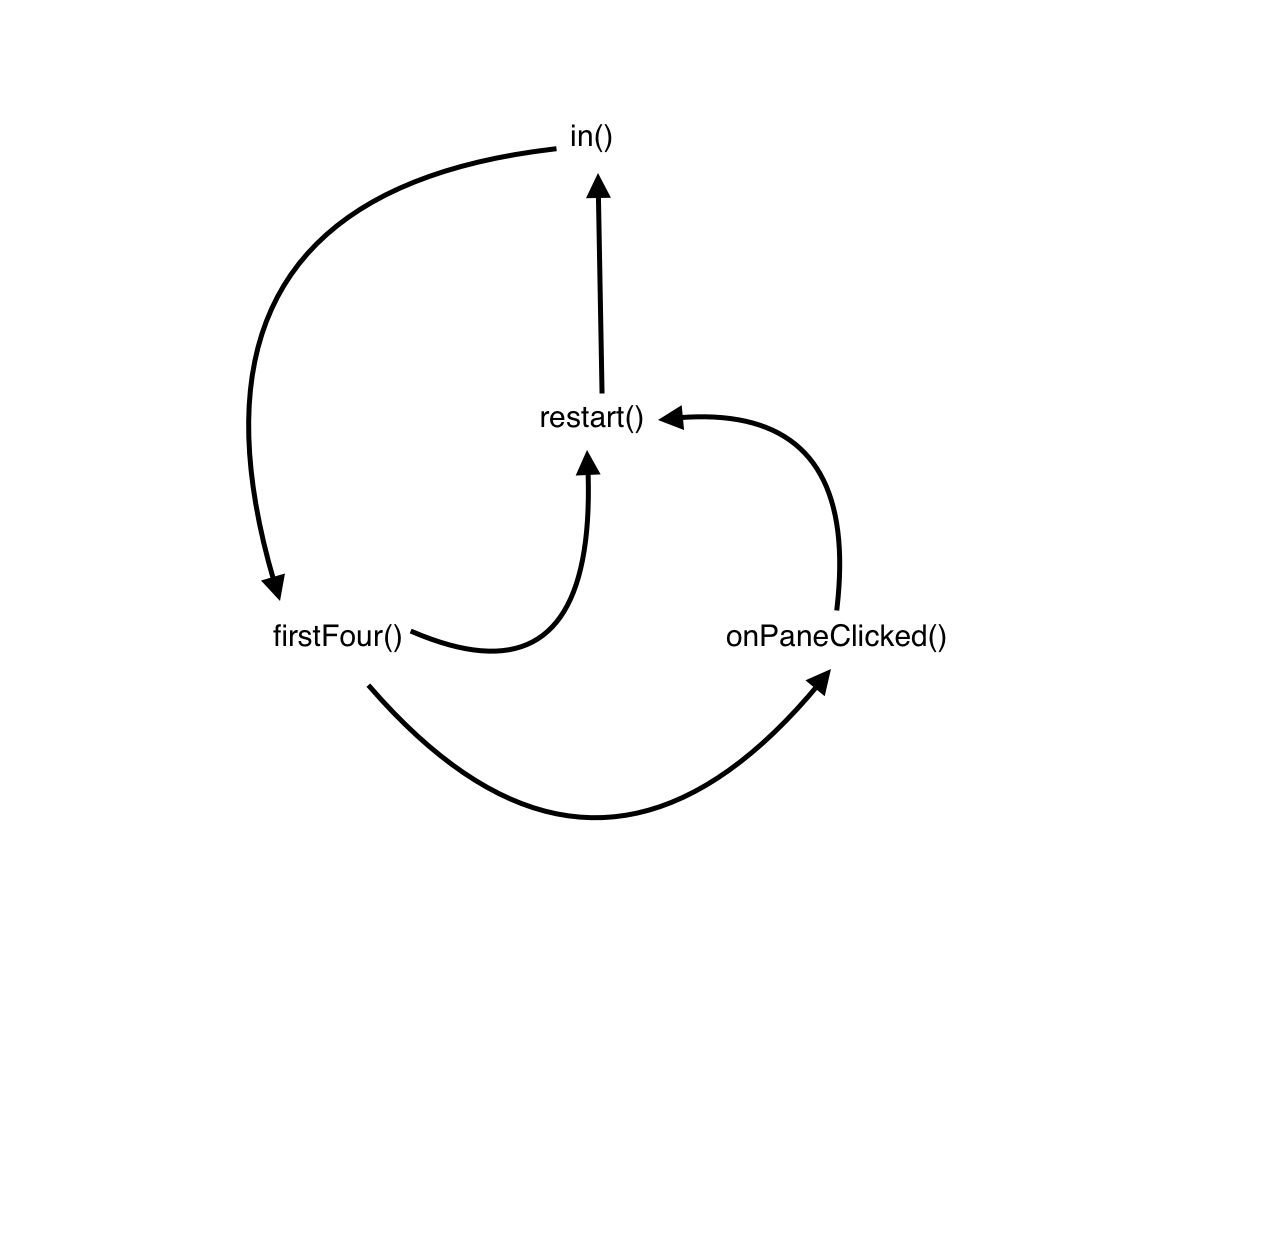
\includegraphics[width=1\textwidth]{Graphics/Basis.png}
\end{figure}
Den røde tråd er meget enkel: spillet igangsættes med metoden 'in()', hvor spillerne bliver tildelt deres farver. Derefter skal den første spiller sætte de første fire brikker ved 'firstFour()'. Nu kan spillerne vælge at genstarte spillet ved 'restart()', i hvilket tilfælde de føres tilbage til 'in()', eller de kan spille videre, hvilket vil føre dem videre til 'onPaneClicked'. Spillet fortsætter, indtil en af afslutningsbetingelserne er opfyldt, hvorefter spillet afsluttes, pointene optælles og vinderen kåres. Nu kan spillerne vælge at genstarte spillet, hvilket tager dem tilbage til 'in()'.

\subsubsection{Avancerede overordnede metoder}\label{AOM}
I den avancerede controller klasse er der rykket om på rækkefølgen, hvori metoderne kaldes. Nedenfor ses en tabel, der viser kronologien af de "overordnede" metoder", samt de metoder, de kalder.
\begin{table}[H]
    \centering
    \caption{Overordnede metoder i Advanced Reversi}\label{tbl:}
    \begin{tabular}{lll}
        \toprule
        Metode          & Kalder metoderne: & Beskrivelse                                                         \\
        \midrule
        beginGame()     & setName()         & Starter spillet og loader Reversibrættet.                                                   \\
                        & \\
                        
        setName()       & setNameBtn()      & Anmoder spillerne om at indtaste deres navne.                                          \\
                        & checkScore()      &                                                                   \\
                        &                   &                                                                   \\

        setNameBtn()    & in()              & Fastlåser navnene til spillerne.                     \\
                        &                                                                                       \\

        in()            & drawCircle()      & Tildeler spillerne deres                                          \\
                        &                   & farver og viser de fire                                           \\
                        &                   & første mulige træk.                                                \\
                        &                   &                                                                   \\

        firstFour()     & update()          & Får spiller nr. 1 til at sætte                                          \\
                        & checkscore()      & de fire første brikker.                                            \\
                        &                                                                                       \\

        onPaneClicked() & getRowIndex()     & Styrer hvad der sker, når                                         \\
                        & getColumnIndex()  & der bliver klikket på et felt.                                   \\
                        & firstFour()       & Annoncerer spillets slutning,                                        \\
                        & hideLegalMoves()  & når der ikke er flere lovlige træk.                                     \\
                        & update()               \\
                        & checkScore()           \\
                        & showLegalMoves()       \\
                        &                        \\

        gameOver()      & loadHighScore()   & Erklærer vinderen                                                 \\
                        & checkHighScore()  & og opdaterer high-score'n                                         \\
                        &                   & (hvis den er blevet slået)                                        \\
                

        \bottomrule
    \end{tabular}
\end{table}


En alternativ repræsentation af metodernes rækkefølge kan vises ved figuren nedenfor:
\begin{figure}[H]
    \centering
    \caption{Advanced Reversi: overordnede metoder}\label{ARF}
    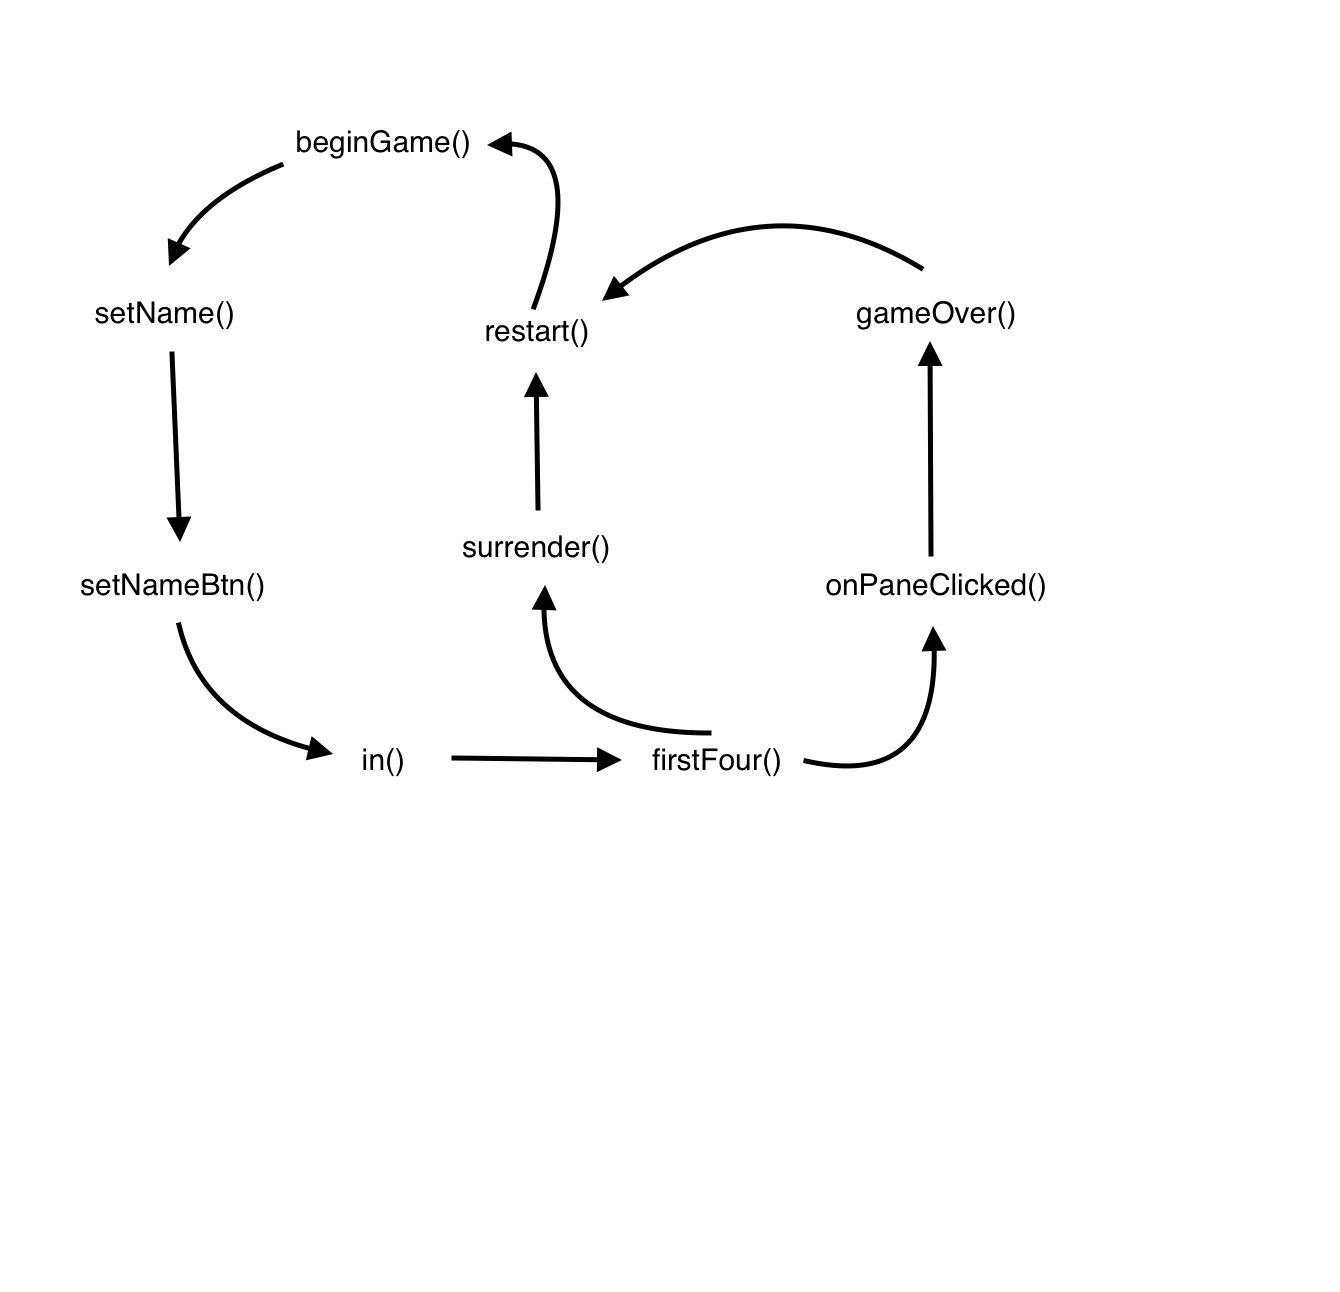
\includegraphics[width=1.2\textwidth]{Graphics/Screenshot 2023-01-20 at 16.35.36.png}
\end{figure}
Her man se, at det hele begynder ved 'beginGame()'. Skriver spillerne deres navne og fortsætter til 'firstFour', hvorefter de nu er i stand til- (men ikke tvunget) at overgive sig, ved at trykke på 'surrender'. Dette vil føre dem til at trykke på 'restart', hvorefter kredsløbet gentager sig. Hvis de ikke giver op, føres de videre til 'onPaneClicked()', som fungerer som spillets "hovedfase", hvor spiller sætter brikker og fylder brættet ud. I sidste ende, når der ikke er flere lovlige træk, sendes spillerne videre til 'gameOver()', hvor pointene tælles op og vinderen kåres.

En metode der er ganske bemærkelsesværdig under controller-klassen er 'beginGame()'. Denne metode, som kaldes ved et tryk på knappen "Begin Game" fra hovedmenuen, igangsætter hele spillet, viser brættet og kalder 'setName()'-metoden. Hvad der er usædvanligt ved denne metode er, at den fungerer ikke just som en controller-metode, der henter data fra 'Board' og bearbejder det. Den fungerer snarer som en metode inde fra 'Main'-klassen, altså klassen der fungerer som "view", hvis vi tager udgangspunkt i MVC-modellen. Den har til job at skulle "vise", men den befinder sig inde i 'controller'-klassen. Grunden til at den befinder sig her, er fordi den kaldes via. en "ActionEvent event", altså kaldes den, når spilleren interagerer manuelt med knappen i hovedmenuen. 

\subsubsection{Avancerede Underordnede Metoder}
\cref{tbl:2}
\begin{table}[H]
    \centering
    \caption{Metoder brugt til avancerede funktioner og i overordnede metoder \mintinline{java}|Avanceret-Controller.java|}\label{tbl:2}
    \begin{tabular}{lll}
        \toprule
        Metode                               & Kaldte metoder  & Beskrivelse                                               \\
        \midrule
        restart(ActionEvent event)           & reset()         & Genstarter spillet og beder spillerene om                 \\
                                             & setName()       & at indsatte deres navne  i tekstfelte igen.               \\
                                             &                 & Spiller der lavet første træk i                           \\
                                             &                 & sidste runde, begynder anden                              \\
                                             &                 &                                                           \\
        reset()                              &                 & Iterer gennem brættet og rydder det                       \\
                                             &                 &                                                           \\
        update()                             & drawCircle()    & Opdatere brættet og tegner circkler(brikker)              \\
                                             &                 & på brættet ifølge Board objektet                          \\
                                             &                 &                                                           \\
        exitGame(ActionEvent event)          &                 & lukker spille                                             \\
                                             &                 &                                                           \\
        checkScore()                         &                 & Opdaterer scoren for begge spillere                       \\
                                             &                 &                                                           \\
        saveHighScore(int score,String name) &                 & Gemmer vinderens score og navnet adskilt af               \\
                                             &                 & komma inde i "Highscore.txt" file, hvis vinderens         \\
                                             &                 & score er højre end nuværende highscore                    \\
                                             &                 &                                                           \\
        loadHighScore()                      &                 & Læser highscore og spillersnavne fra                      \\
                                             &                 & "Highscore.txt" filen og retunere de som arrayet.         \\
                                             &                 &                                                           \\
        showHighScore(ActionEvent event)     & loadHighScore() & Når man trykker på highscore-knappen,                     \\
                                             &                 & vises en advarselsboks/-prompt, der viser highscore       \\
                                             &                 & og spillerens navn, hvis highscore er indstillet.         \\
                                             &                 &                                                           \\
        surrender(ActionEvent event)         &                 & Annoncere overgivelsen af den spiller                     \\
                                             &                 & der trykkede på knappen,                                  \\
                                             &                 & og den anden spillers sejr                                \\
                                             &                 &                                                           \\
        getRowIndex(MouseEvent event)        &                 & Returnerer rækkeindekset for pane, der er klikket på      \\
                                             &                 &                                                           \\
        getColumnIndex(MouseEvent event)     &                 & Returnerer søjleindekset for pane, der er klikket på      \\
                                             &                 &                                                           \\
        showLegalMoves(int color)            & drawCircle()    & Tegner en cirkel hvor spiller kan mulig placer en brik    \\
                                             &                 &                                                           \\
        hideLegalMoves()                     &                 & Rydder brættet for cirkler, hvilket indikerer mulige træk \\
                                             &                 &                                                           \\
        mainMenu(ActionEvent event)          &                 & Returner brugeren tilbage til main-menu af spillet                 \\
        \\
        DrawCircle(int id, Pane pane) & & Tegner hvid og sort brikker og brikker det kan mulig  \\
                         & & placer på brættet, baseret på spillerens tur
                         \\         
        \bottomrule
    \end{tabular}
\end{table}

\subsubsection{Genstarter Spillet} \label{gs}

Et af de grundlæggende kriterier for det basis Reversi-spil er evnen til at genstarte spillet uden at genstarte applikationen. Det er gjort muligt at genstarte spillet uden at genstarte programmet ved at oprette en knap. Genstart-knappen havde oprindelig funktionalitet til at genstarte spillet ved at skifte scener, det vil sige at skifte til scenen, hvor ingen brikker er placeret på brættet. Den tom brættet er den samme scene, der vises ved kørsel af FXML-filen i starten af spillet/programmet. Genstart af spillet med at skifte scener var ikke et optimalt og vellykket middel til at genstarte spillet, da det ikke tillod brugeren at spille spillet igen uden at lukke programm, på grund af det uretmæssige initialisering af spillet samt kun indlæse scenen (tom brættet) med ingen funktionalitet. \newline
\newline
For at undgå denne ukorrekte genstart blev hver pane indeholdt i GridPane tildelt et id (fx: 05 repræsenterer Pane i 0. række og 5. kolonne i GridPane). Hver gang man trykker på genstart, vil to for-loops iterere gennem hver række og kolonne i GridPane, få adgang til den unikke identifikator for hver Pane ved hjælp af række- og kolonneindekset og derefter rydder brikkerne  på den. At tildele et id til ruderne og bruge for -loops til at iterere gennem Pane og slet brikkerne placeret på dem, gav den mest effektive og effektive metode til at genstarte spillet igen. Derudover, når spillet genstartes, vil den spiller, der foretager det første træk, før spillet genstartes, nu starte som nummer to.

